\subsubsection{Which implementation technologies and tools are adopted by software development professionals?}
\label{tools}

Our survey included five questions to find technologies and tools that are adopted by software development professionals. To answer this question fully, we report the following results:
\begin{itemize}
\item Technology Platform (Q 9).
\item Operating System (Q 10).
\item Programming Language (Q 11).
\item Framework (Q 12).
\item IDE (Q 13).
\end{itemize}


\paragraph{Technology Platforms}
Participants were allowed to choose multiple options. As shown in Figure \ref{fig:platforms}, most of our survey respondents (80\%) work in web platform. The rests are mobile (45\%), Desktop (30\%), Embedded/IOT (8\%). This result shows that clients of software products heavily rely on web-based services. 

\begin{figure}[htbp]
\centering
  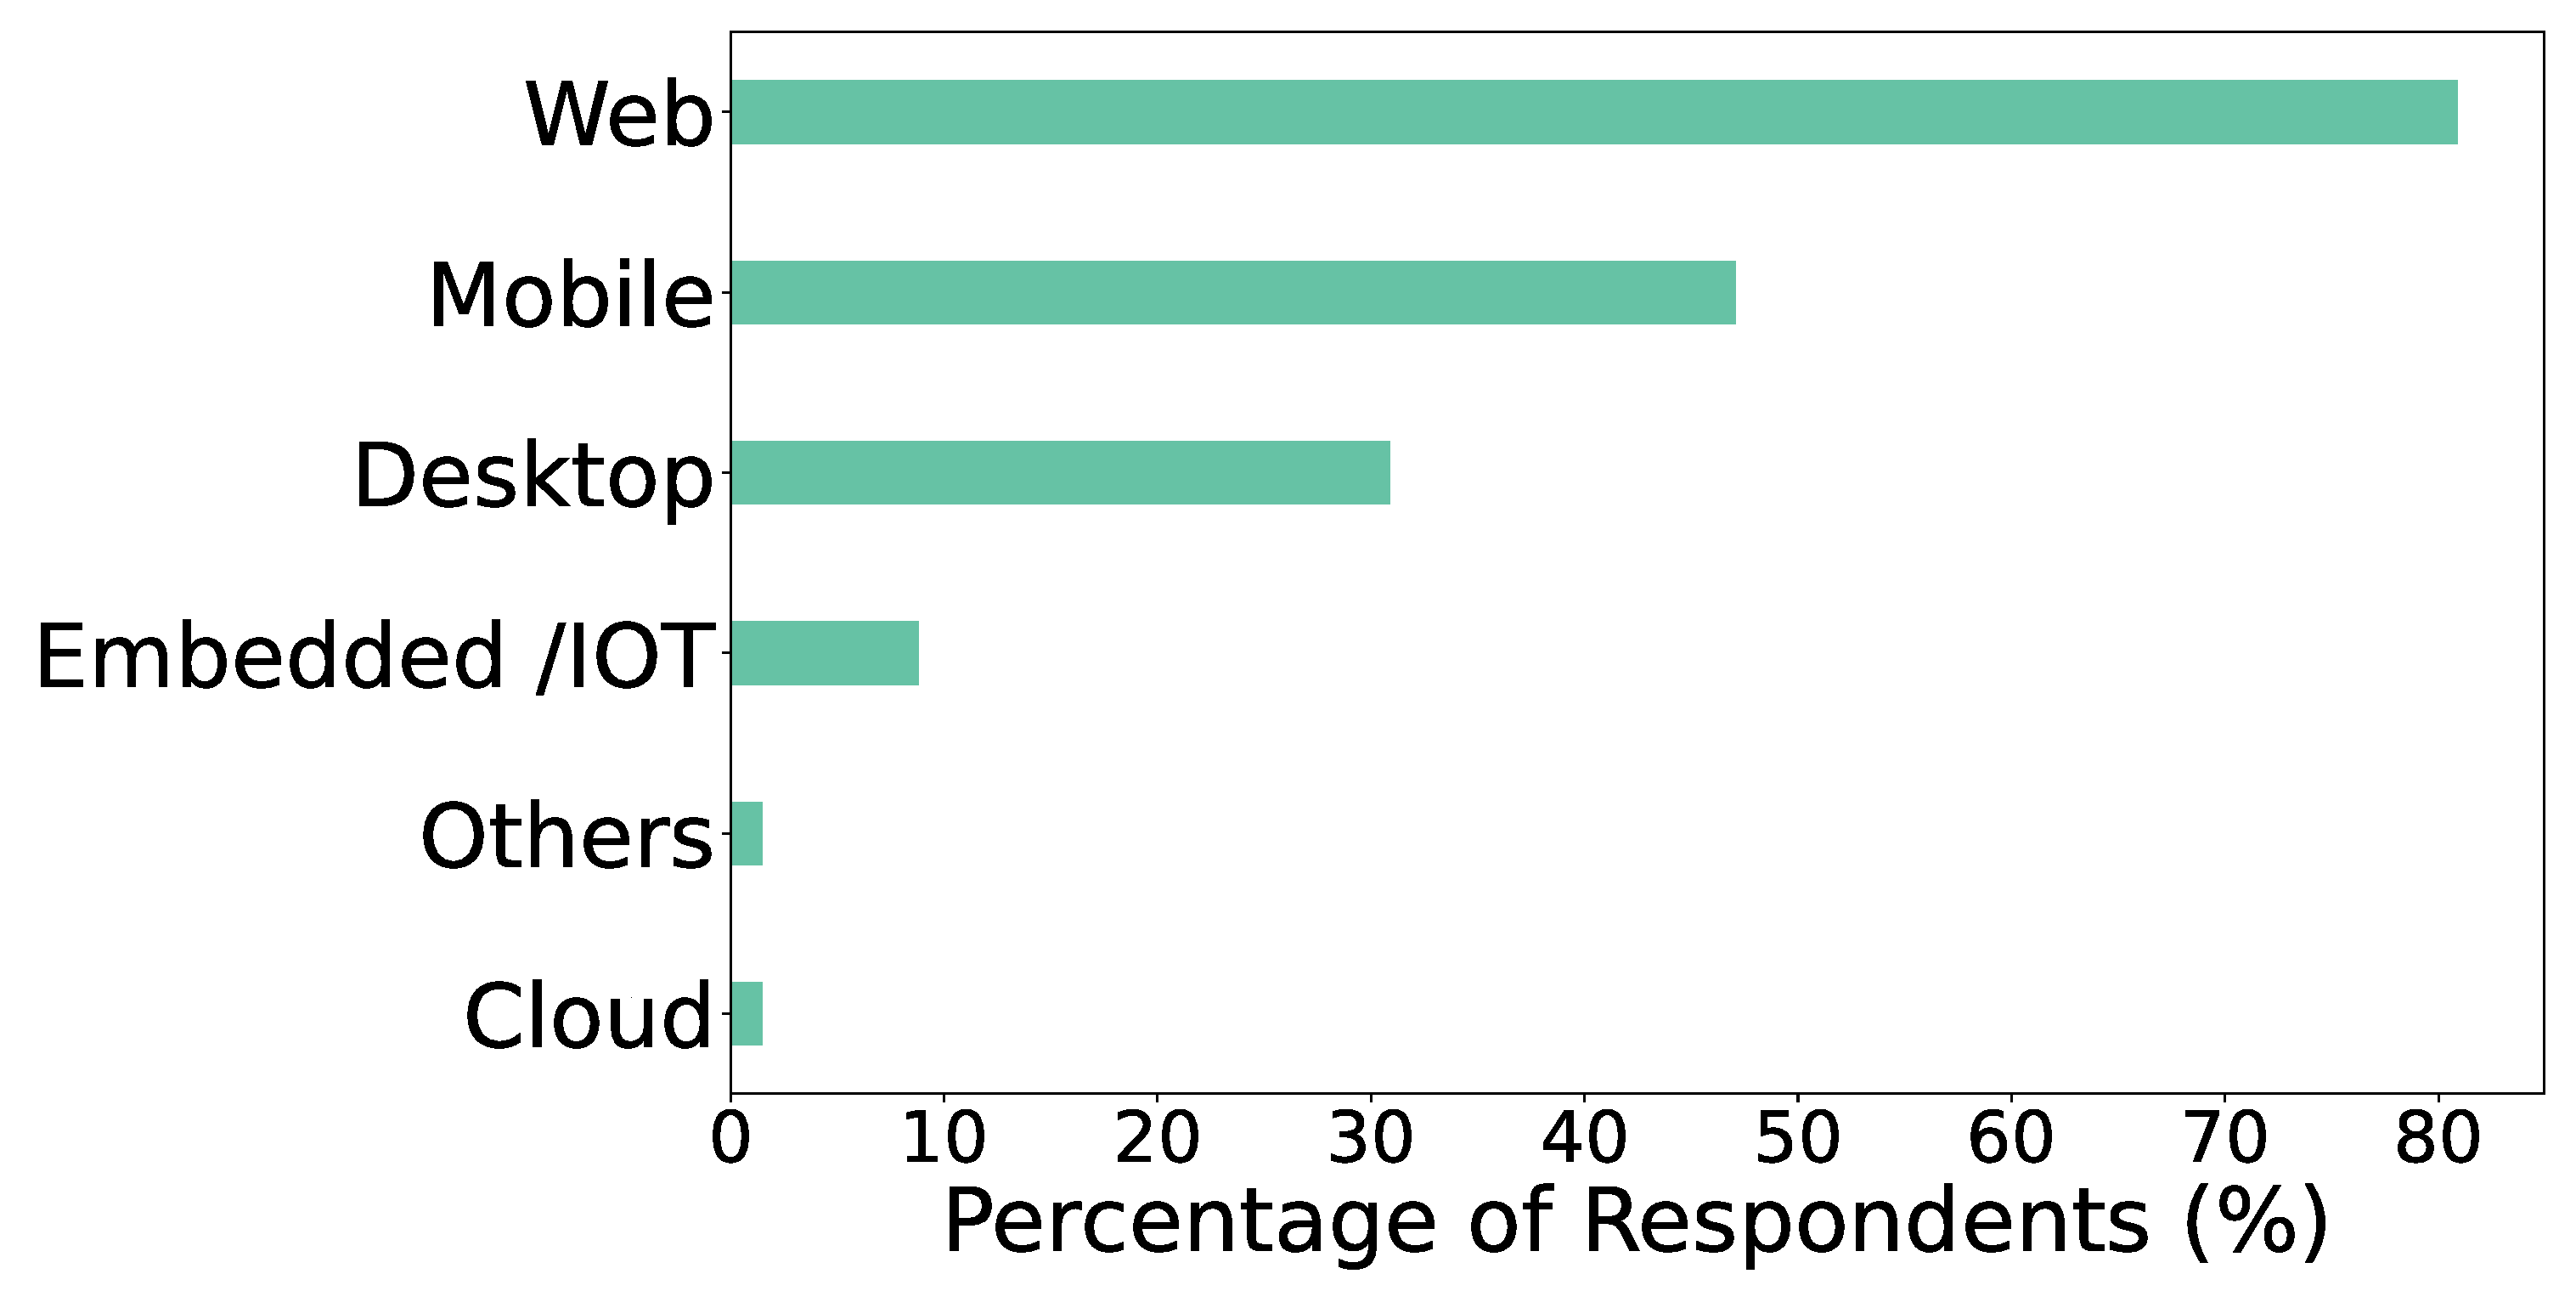
\includegraphics[width=0.8\textwidth]{Figures/Respondents_Technologies}
  \caption{Technology Platforms}
  \label{fig:platforms}
\end{figure}

\boxtext{Web based software services have market demand in a great degree in Bangladesh.}


\paragraph{Operating Systems}
Most of our respondent's use linux based operating system (56\%). The second best used operating system is windows (45\%).

% \begin{figure}[htbp]
% \centering
%   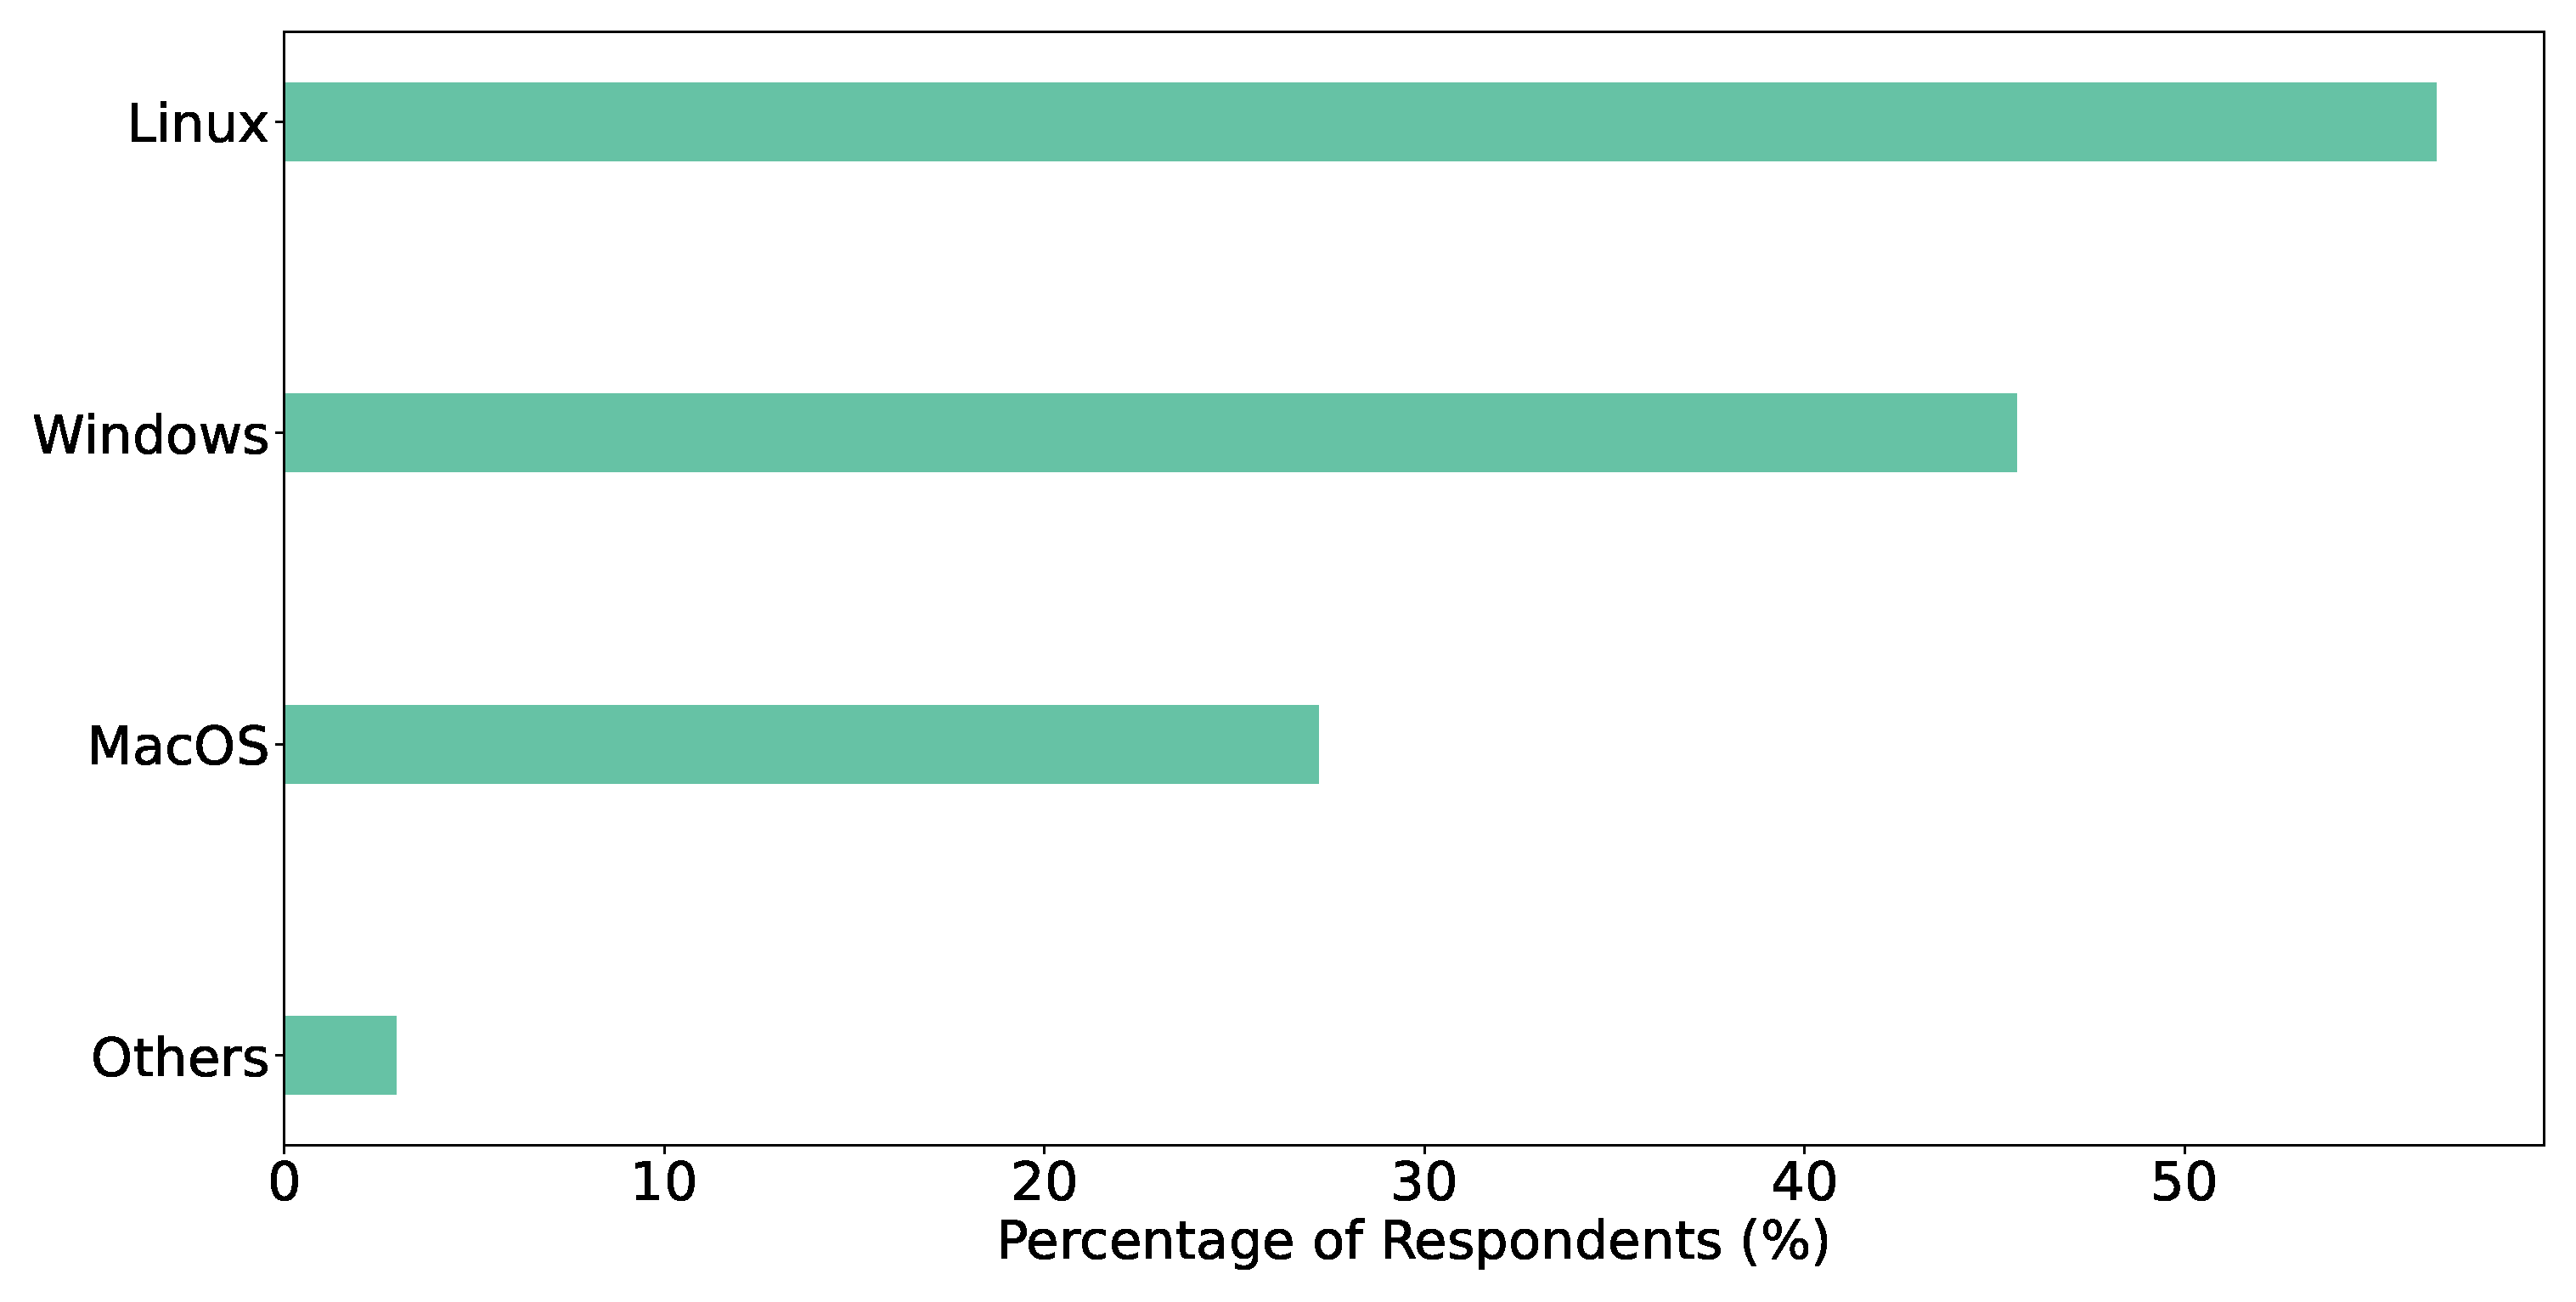
\includegraphics[width=0.8\textwidth]{Figures/Respondents_os}
%   \caption{Operating Systems}
%   \label{fig:os}
% \end{figure}


\paragraph{Programming Languages}
According to \ref{fig:languages}, around 61\% of our respondent's use Java and Javascript each. Other languages like php (25\%), python (25\%), c\# (18\%) are also used which indicates that the software engineers are not inclined towards a single specific language. Also the choice of programming languages used for development can have important inferences for the testing practices of a software company.

% \begin{figure}[htbp]
% \centering
%   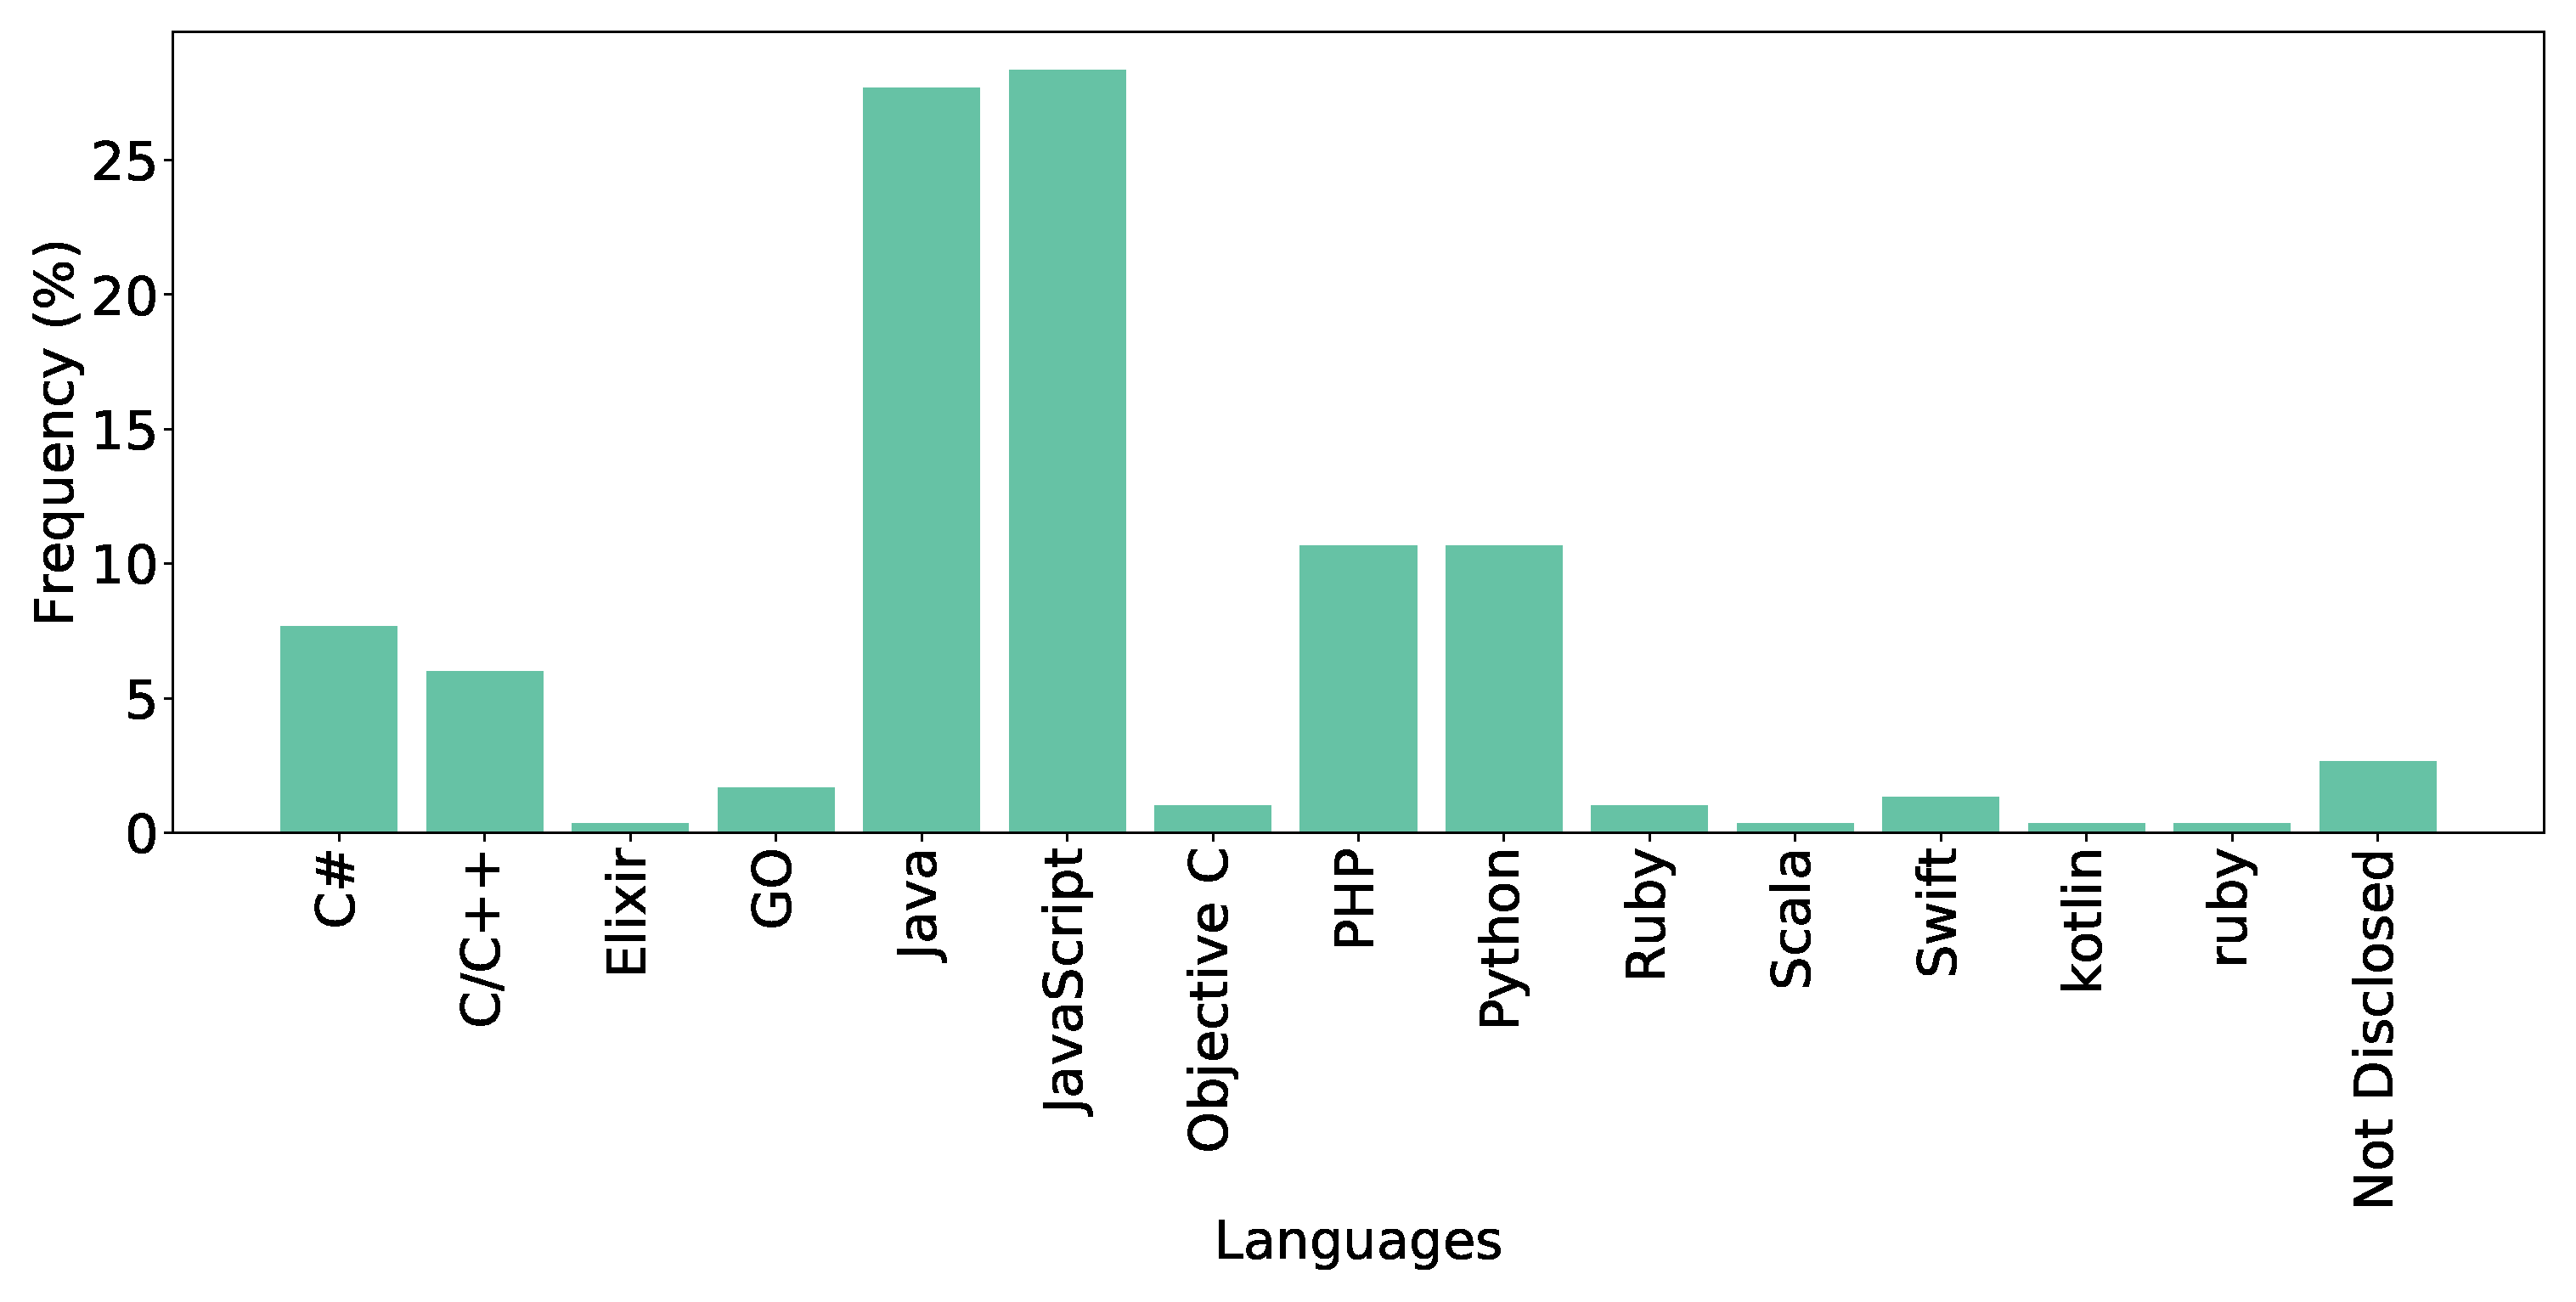
\includegraphics[width=0.8\textwidth]{Figures/Respondents_languages}
%   \caption{Languages used in software development}
%   \label{fig:languages}
% \end{figure}


\paragraph{Frameworks used in development}
As shown in \ref{fig:frameworks}, variety of frameworks have been used during development. Spring boot (37\%) is the mostly used framework in the industry. ASP.NET, Django and Laravel are used in same proportion (14\%).

% \begin{figure}[htbp]
% \centering
%   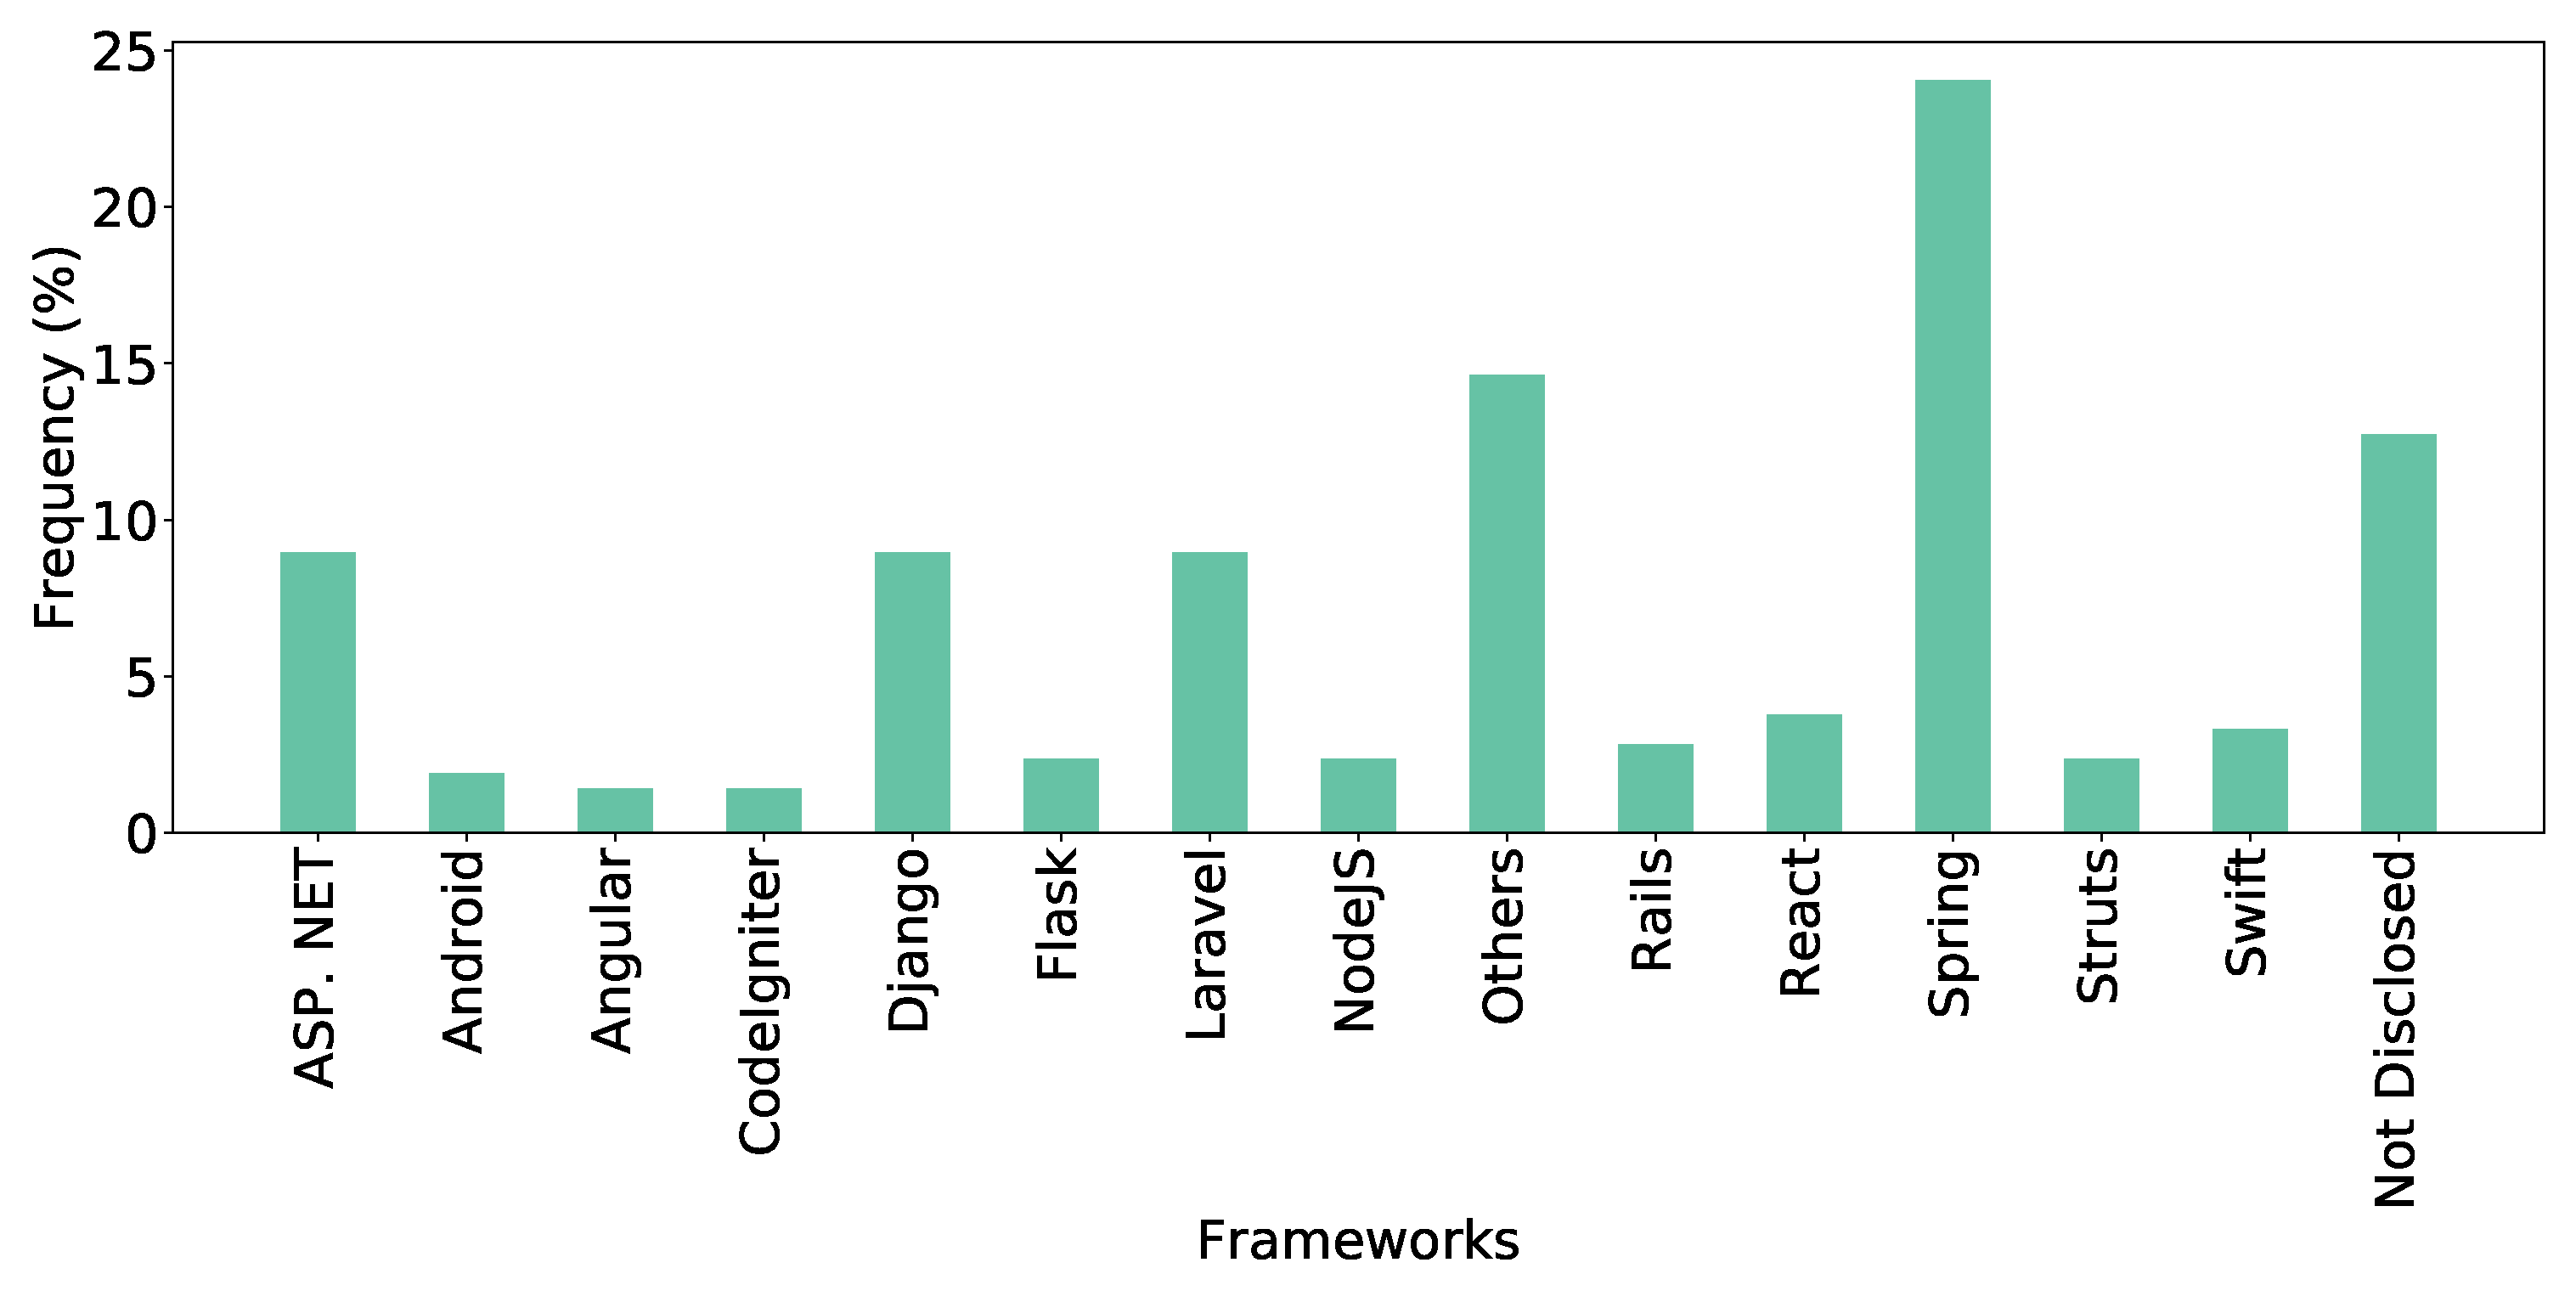
\includegraphics[width=0.8\textwidth]{Figures/Respondents_frameworks}
%   \caption{Frameworks}
%   \label{fig:frameworks}
% \end{figure}


\paragraph{IDE's used by the respondent's}
According to \ref{fig:IDEs}, IntelliJ, a Java integrated development environment for developing computer software for enterprise, mobile, and web development used by most of the respondents (43\%). The other IDEs used in SE industries are: visual studio (30\%), Eclipse (24\%), PyCharm (16\%), NetBeans (10\%), Android Studio (6\%).

% \begin{figure}[htbp]
% \centering
%   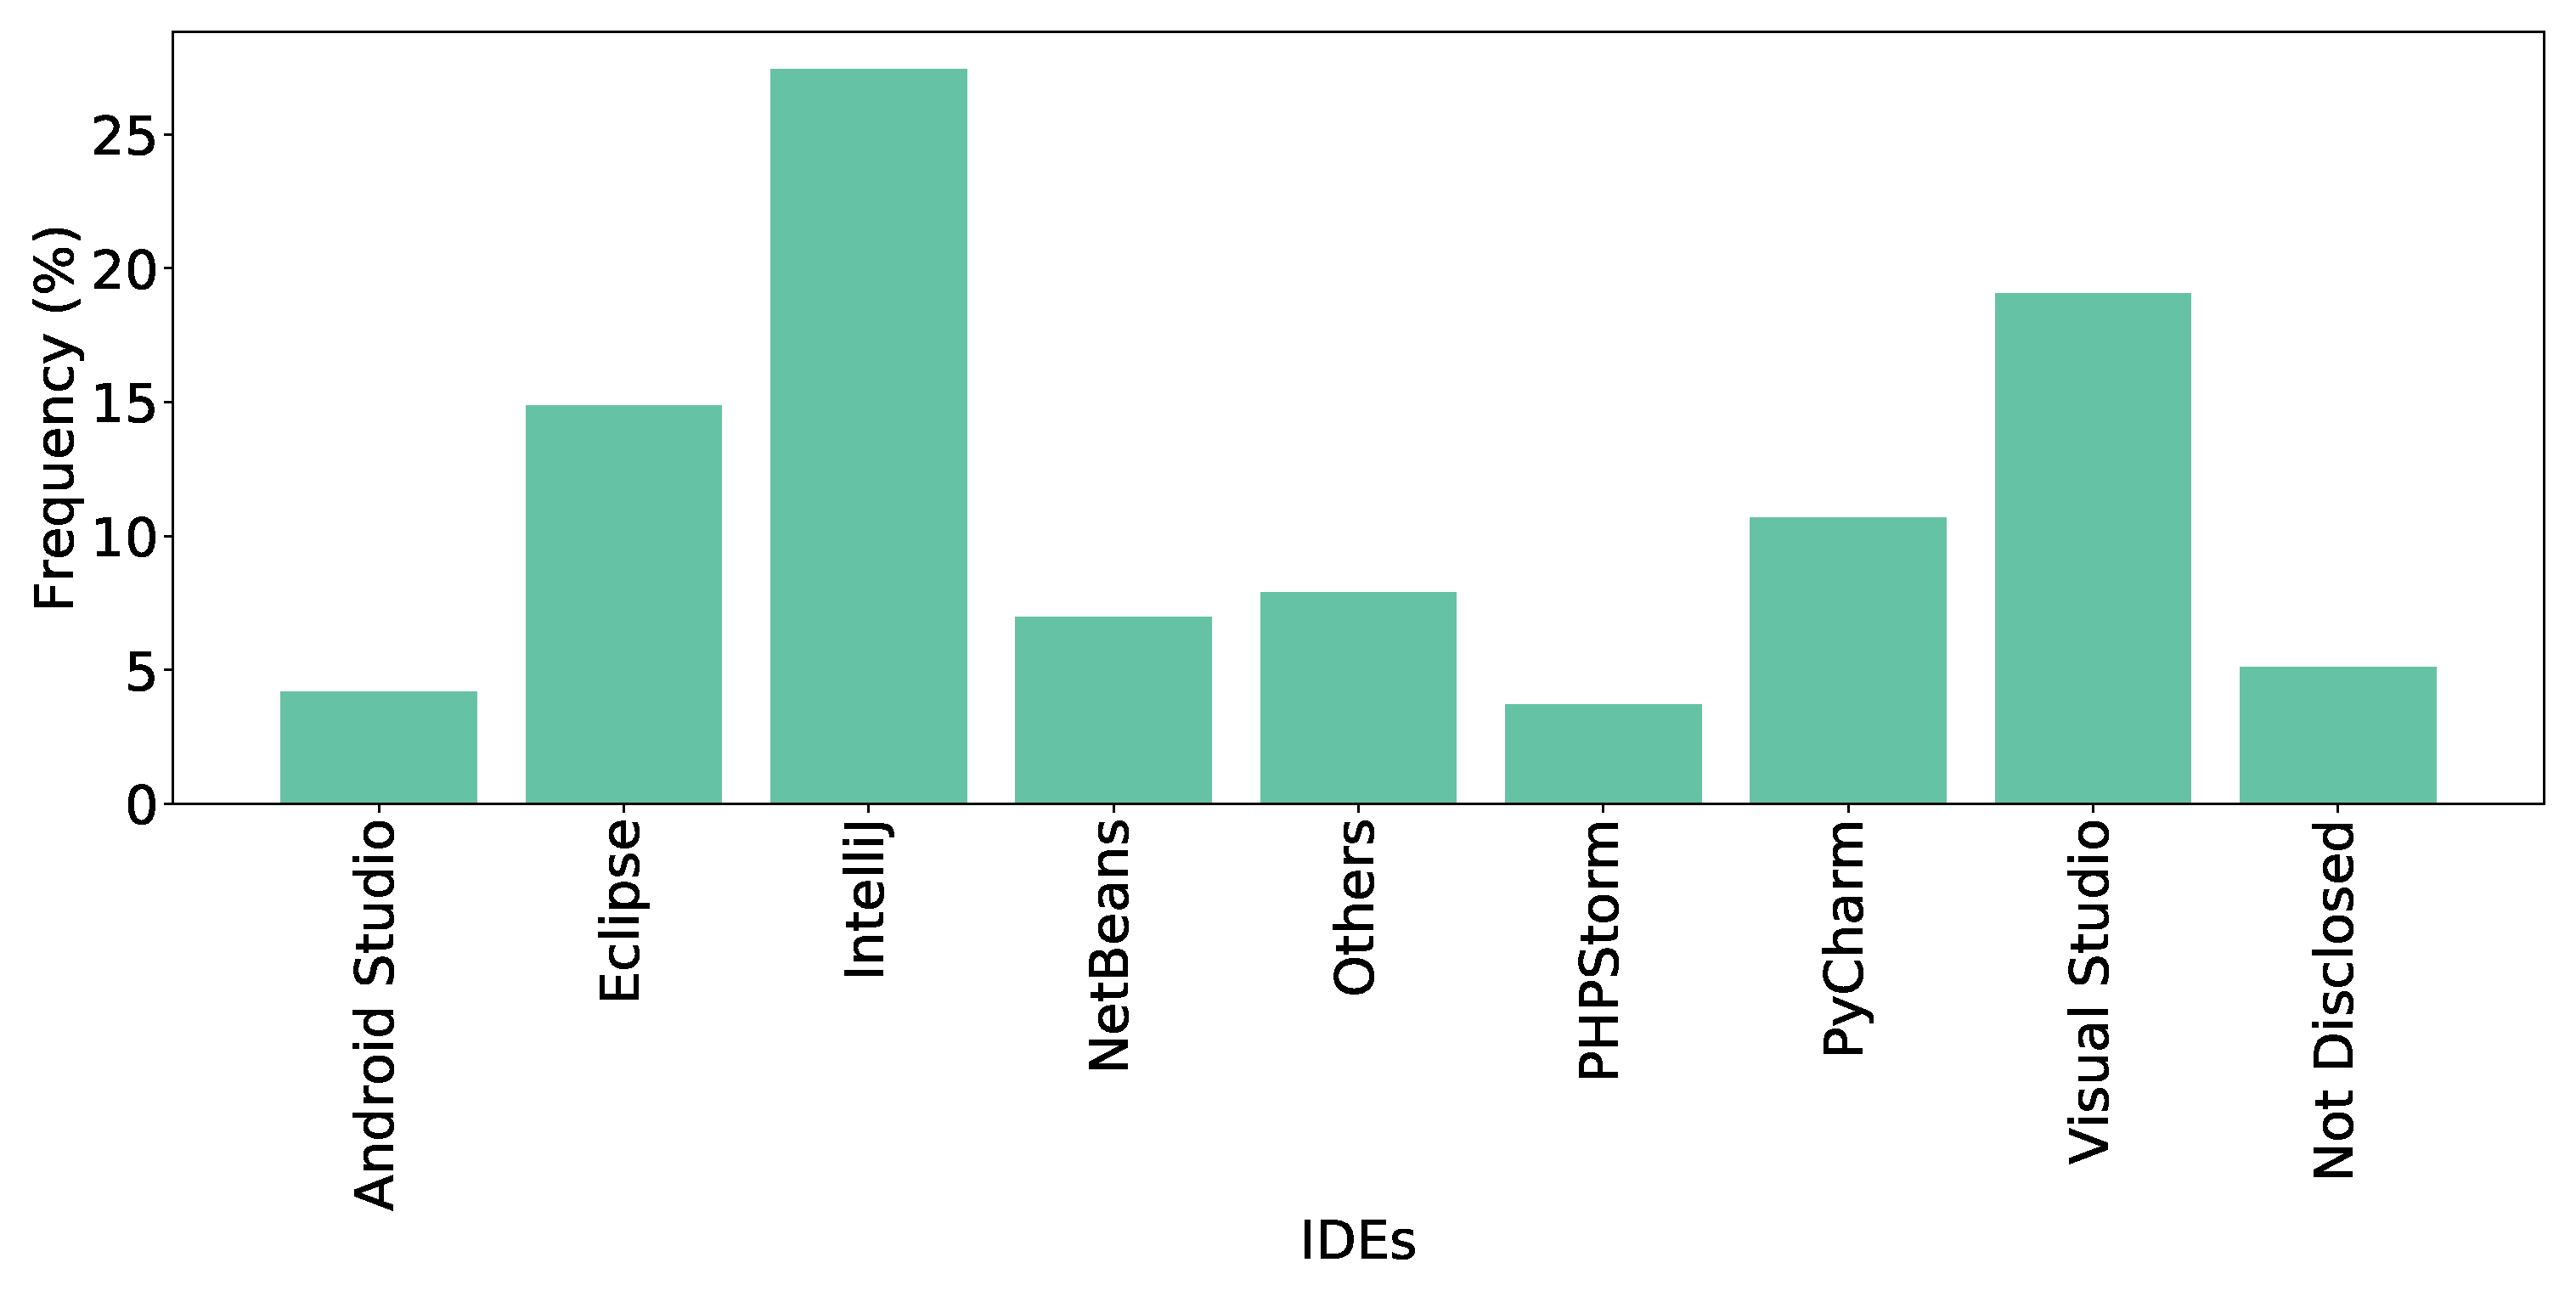
\includegraphics[width=0.8\textwidth]{Figures/Respondents_IDEs}
%   \caption{IDE's}
%   \label{fig:IDEs}
% \end{figure}
